\documentclass[10pt,twocolumn,letterpaper]{article}

\usepackage{cvpr}
\usepackage{times}
\usepackage{epsfig}
\usepackage{graphicx}
\usepackage{amsmath}
\usepackage{amssymb}

% Include other packages here, before hyperref.

% If you comment hyperref and then uncomment it, you should delete
% egpaper.aux before re-running latex.  (Or just hit 'q' on the first latex
% run, let it finish, and you should be clear).
\usepackage[breaklinks=true,bookmarks=false]{hyperref}

\cvprfinalcopy % *** Uncomment this line for the final submission

\def\cvprPaperID{****} % *** Enter the CVPR Paper ID here
\def\httilde{\mbox{\tt\raisebox{-.5ex}{\symbol{126}}}}

% Pages are numbered in submission mode, and unnumbered in camera-ready
%\ifcvprfinal\pagestyle{empty}\fi
\setcounter{page}{1}
\begin{document}

%%%%%%%%% TITLE
\title{COMS W4995 Project Milestone: Automatic Data Augmentation Policy Selection}

\author{Jonathan D. Armstrong\\
{\tt\small jda2160@columbia.edu}
\and
Jesse Galef\\
{\tt\small jbg2160@columbia.edu}
\and
Kyle Matoba\\
{\tt\small km3227@columbia.edu}
}

\maketitle
%\thispagestyle{empty}

%%%%%%%%% ABSTRACT
% \begin{abstract}
% \end{abstract}

% Evaluation metrics for project milestone (20 points)
% Introduction: 2 points
% Related work and references: 2 points
% Problem formulation, technical depth and innovation: 3 points
% Methods, technical depth and innovation, architecture and design: 5 points
% Preliminary results, Github repository, data, code correctness and readability: 8 points
 
%%%%%%%%% BODY TEXT
\section{Introduction}

	For this project, we plan to expand upon the approach used in ``AutoAugment: Learning Augmentation Policies from Data'', \cite{Cubuk2018}. This paper demonstrates success using reinforcement learning to search over a set of possible image transformation policies, finding better ways to augment training data for image classification models. Data augmented according to each combination of transformations explored is used to train a ``child model'', whose performance on a validation set acts as the reward signal for the reinforcement learner. When this data augmentation is combined with state of the art convolutional neural networks (CNNs), such as \cite{Yamada2018} it achieves state of the art results on the CIFAR 10 dataset,\footnote{\url{https://en.wikipedia.org/wiki/CIFAR-10\#Research\_Papers\_Claiming\_State-of-the-Art\_Results\_on\_CIFAR-10}} and several other canonical test problems in image classification. 
	
	We will explore different ways to improve automatic data augmentation using the above paper and their source code as a starting point. Below we propose an ordered set of milestone goals to explore:
	
	\begin{enumerate}

		\item % Reduce Complexity of search space
			A smarter search space: Of the transforms considered, some of them never appeared in any of the policies selected by AutoAugment; we will explore removing these and potentially introducing new transforms that seem promising. Additionally, the authors use only a two-parameter characterization of augmentation (probability of application, and ‘intensity’ when there was such a notion), which can possibly be improved by a more careful understanding of the relevant transforms.
	
		\item % Train a simpler model
			Policy search with a simpler, faster to train model: We may be able to reduce the search time to identify an optimal policy by using a simple model. Once a set of optimal policies is found for this simple model, the same optimal policy should transfer to a state of the art model (trained on the same base dataset).
	
		\item % Fine-grained policies at the category level
			Category-specific policies: there is no reason that different categories within a dataset need to share the same set of invariants. By optimizing policies for each category rather than for the entire dataset, we may be able to further improve accuracy on state of the art models.

	\end{enumerate}

	Using the author's source code, we were able to duplicate their results on CIFAR-10 with several of the smaller architectures, such as a 26 layer ``Shake-Shake`` model of dimension 32 (\cite{Gastaldi2017}) and a Wide Residual Network (\cite{Zagoruyko2016}) with depth 28 and widening factor 10. Note that the authors hard coded the AutoAugment policy into their source code and did not include the code used to generate any of their policies; in other words, the source code is sufficient to validate their results but not to generate new data augmentation policies. In order to proceed, we divided focus into a primary and a naive (backup) approach. 

	The primary approach bakes in concepts from milestone goal 1 and opens the door to exploring goals 2 and 3. This approach involves recreating a reduced version of the AutoAugment procedure and is currently under development.

	The naive approach bakes in concepts from milestone goals 2 and 3: we chose a simple model that can acheive roughly 75\% accuracy and can be trained within 16 minutes using the Google Colaboratory  environment. We are exploring the effects of individual transformation on this model to evaluate how accuracy changes for each image category. Based on these results of this analysis, we intend to create new policies at the image category level to compete against the original AutoAugment code. 

\section{Related works}

	In the transition from machine learning techniques to deep learning, a common theme has emerged: humans are being replaced! Specifically, we are relying less on humans to identify important factors in the data and are now letting our models ``learn'' their own human-independent factors. In this context, it is no surprise that data augmentation is now making the same transition. The canonical approach has been to use a combination of trial and error along with human intuition to select data augmentation policies for a particular dataset. Once a ``reasonable'' set of image transforms have proven successful for a particular dataset, research focus would shift towards model design as the primary means to increase accuracy. The results of the AutoAugment paper have proven that this human-centric approach to data augmentation policy selection falls short when compared to the data-generated policies of their AutoAugment procedure. By training the state of the art models with AutoAugment policies, \cite{Cubuk2018} were able to consistently improve results and able to set a new benchmark. In general, these results demonstrate that data augmentation is indispensable in achieving state of the art performance in image classification. 

	Data augmentation is indispensable in achieving state of the art performance in image classification. This makes  sense, as augmentations can be researched and applied independently of the model architecture, and appear to almost uniformly help. So there's a rough separability -- the best performance will be achieved by the best architecture wedded to the best data augmentation.  One compelling finding to this effect is that \cite{Recht2018} find that out of more than 20 models they entertained, the best-performing model on the CIFAR-10 dataset (\cite{Krizhevsk2009}) was a cutout (\cite{Devries2017}) regularised ``shake-shake'' architecture (\cite{Gastaldi2017}). Cutout is a data augmentation method which appends to the base data set additional occluded images that have had had contiguous regions set to ``zero'' (assuming the data has been normalised around this value). 
	%For example, in \autoref{fig:cutout}, we show a cutout region in a CIFAR 10 image of an ostrich. 
	Not only was the cutout regularized model best in test-set accuracy, but it was also best on the newly-collected ``CIFAR10.1'' dataset with the smallest drop in accuracy. The other well-performing cutout-regularised model, a wide resnet (\cite{Zagoruyko2016}), whilst beaten by some un-augmented models (though the shake-shake model itself has a straightforward interpretation as data augmentation applied to an representation), both in (test) and out of sample, sees a smaller dropoff between CIFAR 10 test and CIFAR10.1 data sets. % Since cutout is not a transform typically used for data augmentation on CIFAR-10 models, the above results imply that with the addition of cutout, model performance is more robust. Note that for the AutoAugment policy for CIFAR-10 3 out of the 95 sub-policies include cutout.

	%\begin{figure}[t]
	%\begin{center}
	%   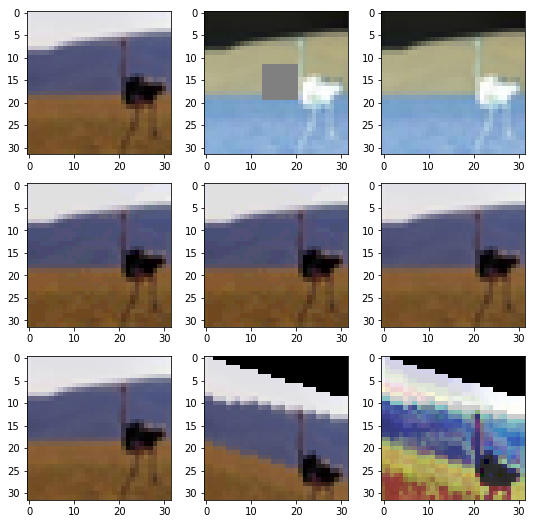
\includegraphics[trim={6.5cm 12.5cm 6.5cm 0}, clip, width=0.8\linewidth]{image.png}
	% <left> <lower> <right> <upper>
	%\end{center}
	%   \caption{A ``cutout`` Bird}
	%\label{fig:cutout}
	%\end{figure}


\section{Preliminary results}

	Using the naive approach we have been able to obtain some preliminary results. First, we have been able to validate our variation of the authors' policy implementation (recall that it was modified to support transforms at the image category level). While our baseline model with no data augmentation can acheive test accuracies roughly between 72 and 74 percent, the same model has achieved 75 percent accuracy when trained with the AutoAugment CIFAR-10 policy. We interpret this as a positive indicator that our policy implementation functions as expected without any critical bugs. Note that training with the AutoAugment policy takes a considerably longer time; the image transformations increase the epoch running time by more than a factor of three and at least 200 epochs are required before validation accuracy plateaus (compared to 50 epochs when trained with no data augmentation). This motivates using a reduced version of the CIFAR-10 training data to continue this analysis
	
	In order to meaningfully compare the effects of using each transform to augment the data, we are exploring the following approach:
	
	\begin{enumerate}
		\item[0)]
			Randomly select 4,000 images from the training data, and use these images as a reduced training set
		
		\item[1)]
			Partially train a baseline model (before the training compression regime occurs)
			
		\item[2)]
			Copy the baseline model and complete training to establish baseline performance with no data augmentation
			
		\item[3)]
			Copy the baseline model and complete training using the AutoAugment policy to establish a competitive accuracy (to try to beat)
			
		\item[4)]
			For each supported image transform (or any combination of interest), copy the baseline model and complete training using the selected transform;
			
	\end{enumerate}
	
	Initial exploration has demonstrated different accuracy responses at the category-level. For example, the translate-Y transform increased the test accuracy of the ``airplane`` category from 48.5\% to 66\%; in the other direction, the cutout transform decreased the test accuracy of the ``frog`` category from 61.8\% to 50.7\%. Accuracy deltas of similar magnitudes do not seem to be uncommon. Further work is necessary, but these results demonstrate that image category-level policies show promise. 


	%If there is one thing we have learned from many years of working data and modeling, it is to solve the apparently simple problems first, because usually they are not as easy as they appear, and often the entire project may turn out to be rethought (multiple times!). 
	%And even on the rare occasion that the easy bits end up being as straightforward as one expects, they often inform the hard bit importantly.
	%That is very much the approach we have taken thus far: we have been working to spec things out and generally understand all of the moving parts, especially the computational ones. This is a project on meta learning, where we are working on the bleeding edge of performance on a fundamental problem, so almost unavoidably some of our work has proven computational challenging. 

	% In my mind, it's better an unsuccessful at improving the state of the art project that runs, is correct, and can be meaninfully and completely analysed, than one which seems to do better on some simplified version of the problem, but we still aren't 100% certain that it runs correctly, and we've not managed to test it on the genuine out of sample data set, etc.
	
	
	% My results have been slowed somewhat by the necessity of learning to use TensorFlow on an industrial scale, for example I took many hours to pick up TensorBoard. 

\subsection{Replicating \cite{Cubuk2018}}
	Replicating the findings of a paper one is attempting to improve upon is a natural starting point. We have done parts of this. More importantly, we have grasped the code and begun making modifications necessary to more fully extend it, such as loading the CIFAR10.1 data set, and generalizing the set of augmentations.

% 	\subsection{}
% 		\begin{itemize}
% 		\item 
% 			I have also checked the the ``CIFAR 10.1'' dataset\footnote{\url{https://github.com/modestyachts/CIFAR-10.1}} is obtainable, loadable, and in a reasonable shape -- it is. Code that solves the inevitable configuration issues is in the ``models'' repo.
% 		\item 
% 			Taught myself how to use tensorboard.
% 		\item 
% 			Have begun figuring out how to use Google Cloud Services. 
% 		\end{itemize}

	\subsection{Hardware Accelerators: GPUs and TPUs}
		\cite{Cubuk2018} was a product of Google Brain, and while it does not demand hundreds of GPU-years to replicate, it does entail significant computation. For even the least-demanding model, a complete fit would have taken about two months on my CPU. By changing it to running on the K80 GPU offered by Google Colaboratory got this down to about 27 hours. 

		Working on Colaboratory presented numerous challenges around persisting data across sessions. This, sadly, consumed considerable effort, but happily seems to now be mostly resolved. 

		Getting the computation time down another order of magnitude would be ideal and basically 100\% sufficient, as it would mean that quick experiments could be done inside of an hour, and the full run, delivering cutting edge results, could be done overnight. This seems plausible with TPUs, given the relative pricing on the Google Cloud Services site.\footnote{\url{https://cloud.google.com/tpu/docs/pricing}} TPUs are really quite expensive, roughly \$5/hour in Europe, thus in less than a day and a half we would consume our allocated budged, thus we are keen to continue using the TPU available through Colaboratory. As well, it seems that the ``shake-drop'' model giving the (\cite{Yamada2018}) best result in \cite{Cubuk2018} (and thus, as far as we are aware, the best result on CIFAR 10), seems exhaust the memory of the standard GPU image on Colaboratory, something I am hoping can be fixed in a move to TPUs as well. 

		Unfortunately, moving from running tensorflow code from GPUs to TPUs is much less straightforward from moving from CPUs to GPUs. Extending the existing code to run on GPUs is another area of ongoing work.
% subsection end (Hardware Accelerators...)
	

\section{Reduced AutoAugment}

	Each policy of data augmentation requires selecting 10 operations, each with one of 16 transformations, 11 discrete probabilities of application, and 10 magnitudes.  The resulting action space has approximately $2.9 \times 10^{31}$ possible actions, making a policy-gradient reinforcement learning approach preferable.One challenge in vanilla policy gradient methods is finding a way to update weights without moving too far from the current policy. Several surrogate loss functions have been designed to encourage or enforce smaller steps, including Trust Region Policy Optimization (TRPO) and now Proximal Policy Optimization (PPO).AutoAugment uses a variant called PPO-Clip, developed by OpenAI \cite{Schulman2017}. PPO-Clip implements a surrogate loss function that includes a clipped term for how much more or less likely the sampled action trajectory would be under the new policy. The AutoAugment controller model samples and scores a batch of policies before using stochastic gradient descent to optimize for this loss function.
	
	In order to achieve our project's aims of refining the policy search space and testing simpler child models, we needed to recreate the AutoAugment reinforcement learning system. So far, we've implemented the following with Keras and Tensorflow:

	\begin{enumerate}
		\item[1)]
			a LSTM-based controller model that produces data augmentation subpolicies
		
		\item[2)]
			a generator which applies the subpolicies to supply batches of augmented cifar10 images
		
		\item[3)]
			a basic convolutional child model which trains on these generators
		
		\item[4)]
			an optimizer which uses vanilla policy-gradient techniques to update the controller model's weights. We're still working to implement the PPO-Clip strategy, to use a better child model, and to find appropriate hyperparameters for the training process.    At the moment, the performance of the child model varies too much and is providing a very noisy signal to the controller.
			
	\end{enumerate}

\section{Link to Github}
	%Currently the work is spread across a few repos, as well as Google Colab notebooks. We will work to consolidate things into a single, cleanly-runnable shape as we approach conclusion.

	\begin{itemize}
	\item \url{https://github.com/kylematoba/deeplearning-project}
	\item \url{https://github.com/kylematoba/models/tree/master/research/autoaugment}
	%\item %\url{https://colab.research.google.com/drive/1qV3vCsjnEcm5a8nRpN40n4qgVKKBzBkd#scrollTo=uiht7wpPPPCP} (also checked into the \texttt{deeplearning-project} repo above)
	%\item \url{https://colab.research.google.com/drive/13GpO9tSqLxflZ9Z2B6RkWMVzfcemW2v7}
	\end{itemize}

% Note that we've not made the repo public, but we have permissioned \texttt{id2305@columbia.edu}, \texttt{id2303@columbia.edu}, \texttt{}

\nocite{Torralba2008}
{\small
\bibliographystyle{ieee}
\bibliography{../biblio}
}

\end{document}

